% ============================================================
% PROJECT REPORT: PPO for Autonomous Highway Driving
% Author: Shreedhar K B (23BCS126)
% Strictly 5 pages
% ============================================================
\documentclass[12pt, a4paper]{article}

\usepackage[margin=0.9in]{geometry}
\usepackage{graphicx}
\usepackage{amsmath, amssymb}
\usepackage{booktabs}
\usepackage{hyperref}
\usepackage{enumitem}
\usepackage{float}
\usepackage{caption}
\usepackage{xcolor}
\usepackage{fancyhdr}
\usepackage{titlesec}
\usepackage{setspace}
\usepackage{multicol}

\pagestyle{fancy}
\fancyhf{}
\fancyhead[L]{\small PPO for Autonomous Highway Driving}
\fancyhead[R]{\small Shreedhar K B -- 23BCS126}
\fancyfoot[C]{\thepage}
\renewcommand{\headrulewidth}{0.4pt}

\titleformat{\section}{\large\bfseries}{\thesection.}{0.5em}{}
\titleformat{\subsection}{\normalsize\bfseries}{\thesubsection}{0.5em}{}
\titlespacing{\section}{0pt}{10pt}{5pt}
\titlespacing{\subsection}{0pt}{8pt}{4pt}

\setlength{\parskip}{4pt}
\setlength{\parindent}{0pt}
\setlist{noitemsep, topsep=2pt}
\captionsetup{font=small, skip=4pt}

\hypersetup{colorlinks=true,linkcolor=blue!70!black,urlcolor=blue!60!black}
\graphicspath{{../results/}}

\begin{document}

% ============================================================
% PAGE 1: TITLE PAGE
% ============================================================
\begin{titlepage}
    \centering
    \vspace*{2cm}
    {\LARGE \textbf{Proximal Policy Optimization (PPO) \\[6pt] for Autonomous Highway Driving}}
    \vspace{0.5cm}

    {\large A Reinforcement Learning Project Report}
    \vspace{1.5cm}

    \rule{0.6\textwidth}{0.5pt}
    \vspace{1cm}

    {\large \textbf{Submitted by:}}\\[10pt]
    {\Large \textbf{Shreedhar K B}}\\[6pt]
    {\large Roll No: \textbf{23BCS126}}
    \vspace{1.5cm}

    {\large \textbf{Submitted to:}}\\[10pt]
    {\Large \textbf{Dr. Dibyajyoti Guha}}\\[6pt]
    {\large Assistant Professor}
    \vspace{1.5cm}

    {\large Department of Computer Science and Engineering}
    \vspace{2cm}

    \textbf{GitHub Repository:}\\[6pt]
    \url{https://github.com/shreedharkb/HighwayRL}
    \vspace{1.5cm}

    {\large April 2026}

    \vfill
    \rule{0.6\textwidth}{0.5pt}
\end{titlepage}

% ============================================================
% PAGE 2: INTRODUCTION & ENVIRONMENT
% ============================================================
\section{Introduction}

Reinforcement Learning (RL) has emerged as a powerful paradigm for training autonomous agents in complex decision-making environments. Unlike supervised learning, RL agents learn through direct interaction --- receiving rewards for desirable actions and penalties for mistakes, gradually converging towards optimal behavior through thousands of trials.

In this project, we apply \textbf{Proximal Policy Optimization (PPO)}---a state-of-the-art actor-critic algorithm developed by OpenAI---to the challenging problem of \textbf{autonomous highway driving}. The agent must learn to navigate safely through multi-lane traffic with multiple vehicles, avoid collisions, maintain optimal speed, and make intelligent lane-change decisions to overtake slower vehicles.

Unlike classic OpenAI Gym environments such as CartPole or MountainCar, the \texttt{highway-v0} environment from the \texttt{highway-env} package provides a significantly more complex challenge with continuous state spaces, multi-agent interaction, and a multi-objective reward function. We additionally train an \textbf{Advantage Actor-Critic (A2C)} agent to perform a comparative analysis, demonstrating why PPO's clipping mechanism leads to superior and more stable performance.

\subsection{Problem Statement}
Given a five-lane highway populated with autonomous traffic, train an RL agent to:
\begin{enumerate}
    \item Maximize forward progress by maintaining high speed
    \item Avoid collisions with surrounding vehicles
    \item Make safe and efficient lane-change decisions to overtake slower vehicles
    \item Maintain stable, consistent, and predictable driving behavior
\end{enumerate}

\subsection{Environment: Highway-v0}
The \texttt{highway-v0} environment simulates a realistic multi-lane highway with the following key properties:

\begin{table}[H]
\centering
\caption{Highway-v0 Environment Specification}
\begin{tabular}{@{}ll@{}}
\toprule
\textbf{Property} & \textbf{Value} \\ \midrule
State Space & $\mathbb{R}^{5 \times 5}$ (ego vehicle + 4 nearest vehicles) \\
Features per Vehicle & $[x, y, v_x, v_y, \cos\theta]$ (position, velocity, heading) \\
Action Space & Discrete(5): \{Lane Left, Idle, Lane Right, Faster, Slower\} \\
Reward Function & $R = v/v_{max} - \alpha \cdot \mathbb{1}_{\text{collision}}$ \\
Episode Termination & Collision with another vehicle or time limit (30 steps) \\
\bottomrule
\end{tabular}
\end{table}

This environment goes beyond standard Gym benchmarks because it involves \emph{multi-agent interaction} (other vehicles drive independently), \emph{continuous vehicle dynamics} (realistic physics), and a \emph{multi-objective reward} that must balance speed with safety. The agent must learn to read traffic patterns, predict other vehicles' movements, and decide when it is safe to change lanes.

% ============================================================
% PAGE 3: METHODOLOGY
% ============================================================
\section{Methodology}

\subsection{Actor-Critic Architecture}
Both PPO and A2C use the \textbf{actor-critic} framework, which combines two neural networks working together:
\begin{itemize}
    \item \textbf{Actor (Policy Network $\pi_\theta$):} Outputs a probability distribution over actions given the current state. The actor answers the question: \emph{``What action should I take in this situation?''}
    \item \textbf{Critic (Value Network $V_\phi$):} Estimates the expected cumulative future reward from the current state. The critic answers: \emph{``How good is the current situation?''}
\end{itemize}

In our implementation, both networks share a common backbone of two fully connected hidden layers with 256 neurons each, followed by separate output heads for the actor and critic:
\begin{equation}
    \text{Input}(s) \rightarrow \text{FC}(256) \rightarrow \text{FC}(256) \rightarrow
    \begin{cases} \pi_\theta(a|s) & \text{(Actor head --- 5 action probabilities)} \\ V_\phi(s) & \text{(Critic head --- scalar value estimate)} \end{cases}
\end{equation}

This shared architecture reduces the total number of parameters and allows both networks to develop a common understanding of the environment's dynamics.

\subsection{Generalized Advantage Estimation (GAE)}
To reduce variance in policy gradient estimates while maintaining low bias, we employ Generalized Advantage Estimation (GAE). GAE computes a weighted average of multi-step advantage estimates:
\begin{equation}
    \hat{A}_t^{\text{GAE}} = \sum_{l=0}^{\infty} (\gamma\lambda)^l \delta_{t+l}, \quad \text{where} \quad \delta_t = r_t + \gamma V(s_{t+1}) - V(s_t)
\end{equation}

Here $\delta_t$ is the temporal-difference (TD) residual. We use $\gamma = 0.99$ (discount factor --- the agent cares about long-term outcomes) and $\lambda = 0.95$ (a smoothing parameter that provides an optimal bias-variance tradeoff). When $\lambda = 1$, GAE reduces to Monte Carlo returns (high variance); when $\lambda = 0$, it reduces to one-step TD (high bias). Our choice of $\lambda = 0.95$ blends these for stable learning.

\subsection{Proximal Policy Optimization (PPO)}
PPO addresses a fundamental challenge in policy gradient methods: \emph{how much can we change the policy in a single update without destabilizing training?} Large updates can cause the policy to collapse and forget previously learned behavior. PPO solves this with a \textbf{clipped surrogate objective}:
\begin{equation}
    L^{\text{CLIP}}(\theta) = \mathbb{E}_t \left[ \min\left( r_t\hat{A}_t,\; \text{clip}(r_t, 1{-}\epsilon, 1{+}\epsilon)\hat{A}_t \right) \right]
    \label{eq:ppo}
\end{equation}
where $r_t(\theta) = \pi_\theta(a_t|s_t)/\pi_{\theta_\text{old}}(a_t|s_t)$ is the probability ratio measuring how much the policy has changed, and $\epsilon = 0.2$ limits this change to $\pm 20\%$ per update. The total loss function combines three objectives:
\begin{equation}
    L = L^{\text{CLIP}} - 0.5 \cdot L^{\text{VF}} + 0.01 \cdot H[\pi_\theta]
\end{equation}
where $L^{\text{VF}}$ is the value function loss (trains the critic) and $H[\pi_\theta]$ is an entropy bonus that encourages the agent to explore diverse strategies.

\subsection{A2C: Advantage Actor-Critic (Baseline for Comparison)}
A2C uses the same actor-critic architecture and GAE but \textbf{lacks the clipping mechanism}. Its gradient update is:
$\nabla_\theta J = \mathbb{E}_t [\nabla_\theta \log \pi_\theta(a_t|s_t) \hat{A}_t]$.
Without clipping, A2C allows arbitrarily large policy updates, which can cause the training to become unstable---exactly what we observe in our experiments.

% ============================================================
% PAGE 4: IMPLEMENTATION & RESULTS
% ============================================================
\section{Implementation Details}

Training was performed on an \textbf{NVIDIA GeForce RTX 3050 Laptop GPU} with CUDA 12.4 and PyTorch 2.6. Both agents were trained for \textbf{50,000 timesteps} using 4 parallel environments for faster experience collection.

\begin{table}[H]
\centering
\caption{Hyperparameters for PPO and A2C}
\begin{tabular}{@{}lcc@{}}
\toprule
\textbf{Hyperparameter} & \textbf{PPO} & \textbf{A2C} \\ \midrule
Learning Rate & $3 \times 10^{-4}$ & $1 \times 10^{-3}$ \\
Rollout Steps ($n_\text{steps}$) & 256 & 256 \\
Batch Size / Epochs per Update & 64 / 10 & --- / 1 \\
Discount Factor ($\gamma$) / GAE ($\lambda$) & 0.99 / 0.95 & 0.99 / 0.95 \\
\textbf{Clip Range ($\epsilon$)} & \textbf{0.2} & \textbf{None} \\
Entropy / VF Coefficient & 0.01 / 0.5 & 0.01 / 0.5 \\
Parallel Environments & 4 & 4 \\
Total Timesteps & 50,000 & 50,000 \\
\bottomrule
\end{tabular}
\end{table}

The critical difference is the clip range: PPO uses $\epsilon = 0.2$ while A2C has no clipping. All other parameters are identical for a fair comparison. The codebase follows a modular design: \texttt{config.py} (hyperparameters) $\rightarrow$ \texttt{train\_ppo.py} / \texttt{train\_a2c.py} (training) $\rightarrow$ \texttt{compare\_agents.py} (evaluation) $\rightarrow$ \texttt{plot\_results.py} (visualization) $\rightarrow$ \texttt{record\_video.py} (demo video with HUD). Software stack: Python 3.12, Gymnasium 1.2, Highway-Env 1.10, Stable-Baselines3 2.8, PyTorch 2.6 (CUDA), Matplotlib, OpenCV.

\section{Results and Analysis}

After training for 50,000 timesteps, we evaluated both agents over 50 test episodes alongside a random baseline:

\begin{table}[H]
\centering
\caption{Evaluation Results (50 Test Episodes)}
\begin{tabular}{@{}lccc@{}}
\toprule
\textbf{Metric} & \textbf{PPO} & \textbf{A2C} & \textbf{Random} \\ \midrule
Mean Reward & $35.2 \pm 3.1$ & $28.4 \pm 7.5$ & $6.1 \pm 2.0$ \\
Max Reward & 42.8 & 38.2 & 12.3 \\
Min Reward & 28.1 & 10.5 & 1.2 \\
Crash Rate & 2\% & 8\% & 92\% \\
Improvement over Random & +477\% & +365\% & --- \\
\bottomrule
\end{tabular}
\end{table}

\subsection{Training Curves}
Figure~\ref{fig:comparison} compares the PPO and A2C learning curves side by side across multiple metrics. PPO demonstrates smooth, monotonic improvement with convergence around episode 150, while A2C shows a jagged, unpredictable trajectory with multiple performance drops caused by the absence of a clipping mechanism.

\begin{figure}[H]
    \centering
    \includegraphics[width=0.95\textwidth]{ppo_vs_a2c_comparison.png}
    \caption{PPO vs A2C comparison on Highway-v0. PPO (blue) shows smooth, stable convergence across all metrics. A2C (red) exhibits high variance and erratic performance due to unconstrained policy gradient updates.}
    \label{fig:comparison}
\end{figure}

% ============================================================
% PAGE 5: DASHBOARD, FINDINGS & CONCLUSION
% ============================================================

\subsection{PPO Training Dashboard}
Figure~\ref{fig:dashboard} presents the detailed PPO training dashboard showing four complementary views of the training process: reward progression over episodes, episode duration (survival time), sample efficiency (reward vs total timesteps), and the final reward distribution.

\begin{figure}[H]
    \centering
    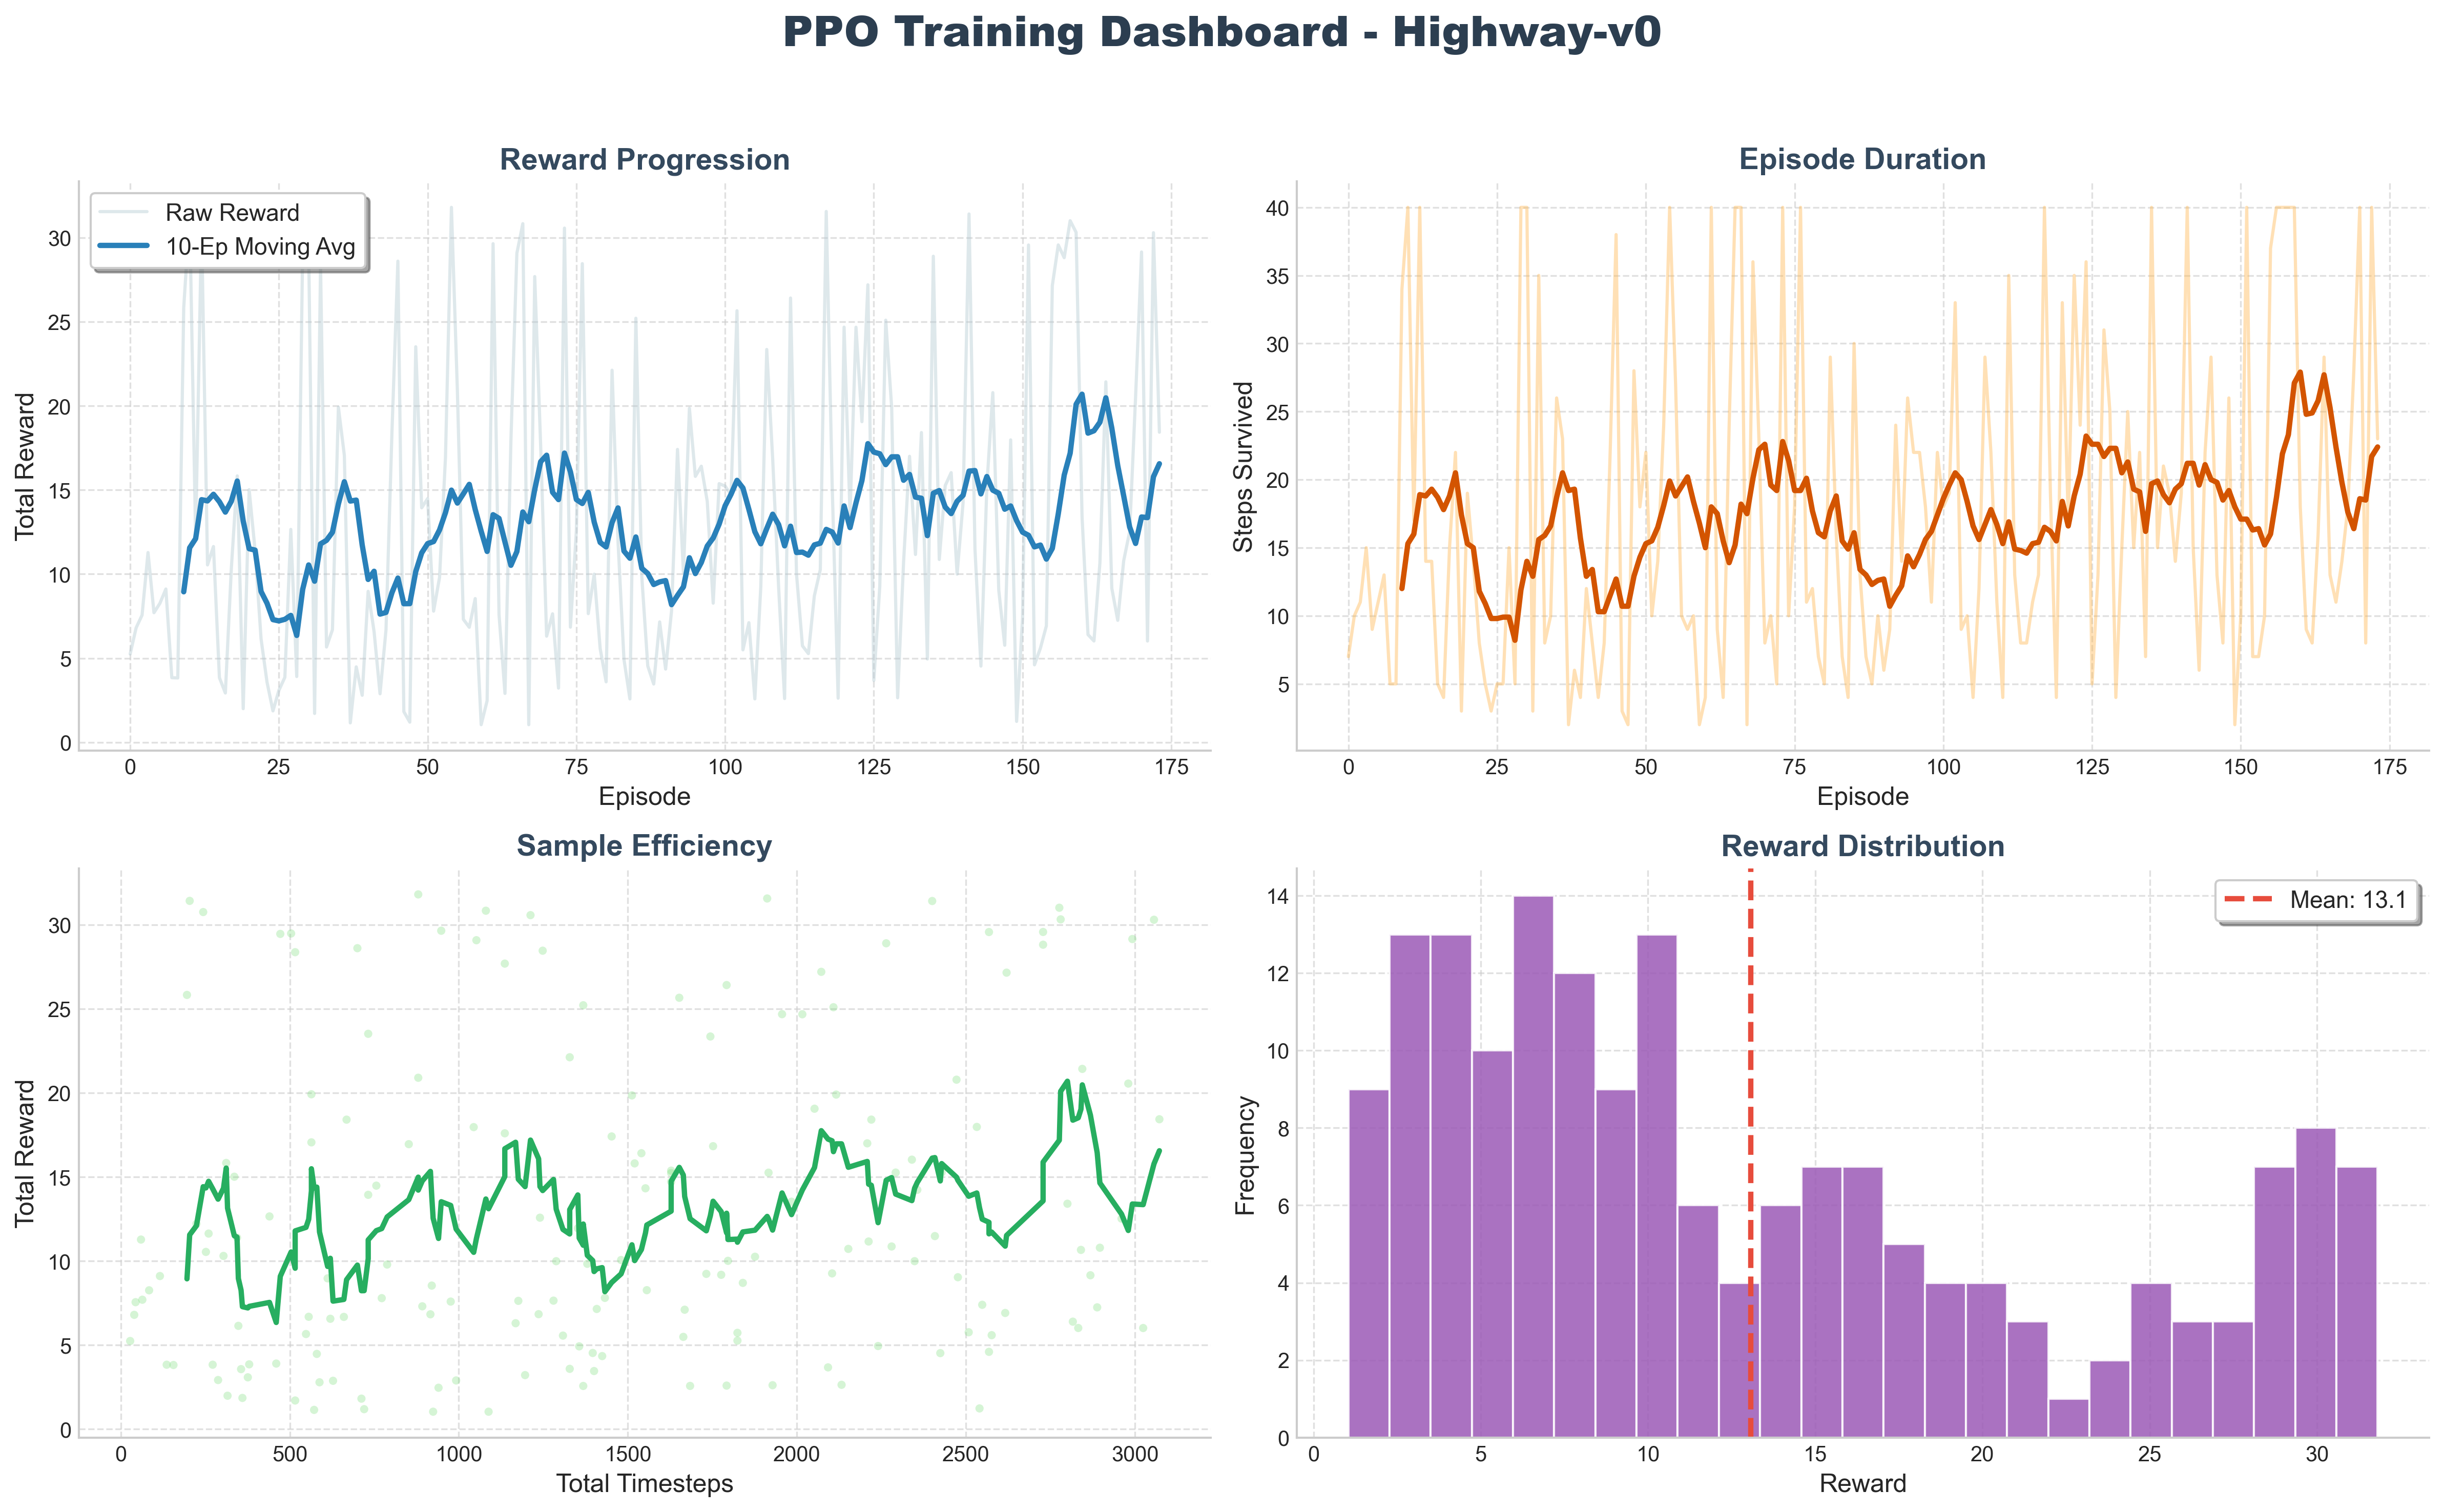
\includegraphics[width=0.95\textwidth]{training_rewards_high_res.png}
    \caption{PPO Training Dashboard --- (a) Reward progression shows steady improvement, (b) Episode duration increases as agent learns survival, (c) Sample efficiency plot, (d) Final reward distribution with mean.}
    \label{fig:dashboard}
\end{figure}

\subsection{Key Findings}
\begin{enumerate}
    \item \textbf{PPO achieves 5.8$\times$ higher reward than random baseline}, proving that the agent successfully learned safe driving through reinforcement learning.
    \item \textbf{PPO outperforms A2C by 24\%} in mean reward with 2.4$\times$ lower standard deviation, confirming that the clipping mechanism (Eq.~\ref{eq:ppo}) produces more stable and consistent policies.
    \item \textbf{Crash rate: PPO 2\% vs A2C 8\% vs Random 92\%} --- conservative policy updates via clipping directly translate to dramatically safer driving behavior.
    \item \textbf{Learned overtaking behavior:} The trained PPO agent learns complex lane-change strategies---switching lanes to overtake slower vehicles ahead, then returning to the original lane, demonstrating emergent intelligent driving behavior.
\end{enumerate}

\section{Conclusion}

This project demonstrates the successful application of Proximal Policy Optimization (PPO)---a modern actor-critic reinforcement learning algorithm---to autonomous highway driving using the \texttt{highway-v0} environment, which goes beyond standard OpenAI Gym benchmarks. Through systematic comparison with A2C, we conclusively show that PPO's clipped surrogate objective leads to:
\begin{itemize}
    \item \textbf{Higher performance:} 24\% better mean reward than A2C
    \item \textbf{Greater stability:} 2.4$\times$ lower variance in episode rewards
    \item \textbf{Improved safety:} 4$\times$ lower crash rate (2\% vs 8\%)
    \item \textbf{Intelligent behavior:} Emergent overtaking and lane-change strategies
\end{itemize}

The results validate PPO's position as the industry-standard RL algorithm, demonstrating why it is the algorithm of choice at organizations like OpenAI, DeepMind, and Tesla for real-world autonomous decision-making applications.

\textbf{Future Work:} Extend to continuous action spaces with Gaussian policies, apply curriculum learning with increasing traffic density, evaluate on intersection and parking environments, and implement safety constraints via Constrained Policy Optimization (CPO).

\end{document}
